\section{Overview Analysis of Relevant Market Systems}

\subsection{Library Resource Management and Search System -- Ho Chi Minh City University of Technology (HCMUT)}

The library resource management and search system at Ho Chi Minh City University of Technology (VNU-HCM) currently operates through two independent yet complementary component portals: the Official Library Information Portal (\url{https://lib.hcmut.edu.vn/}) and the Online Public Access Catalog system (OPAC at \url{https://opac.lib.hcmut.edu.vn/}). This combination aims to manage and serve two core resource streams in parallel: traditional printed materials and institutional repository assets.

For the main library information portal (\url{lib.hcmut.edu.vn}), the system serves as a central hub managing and presenting all print materials, including textbooks, reference books, and academic journals across various disciplines physically stored in campus stacks (such as the Loan Collection in Building B2, Reference Collection in Building B4 at Ly Thuong Kiet Campus, and the Library at Di An Campus). Users on this interface primarily access general announcements, loan rules, or utilize the quick search bar to verify the physical availability of print volumes.

\begin{figure}[H]
    \centering
     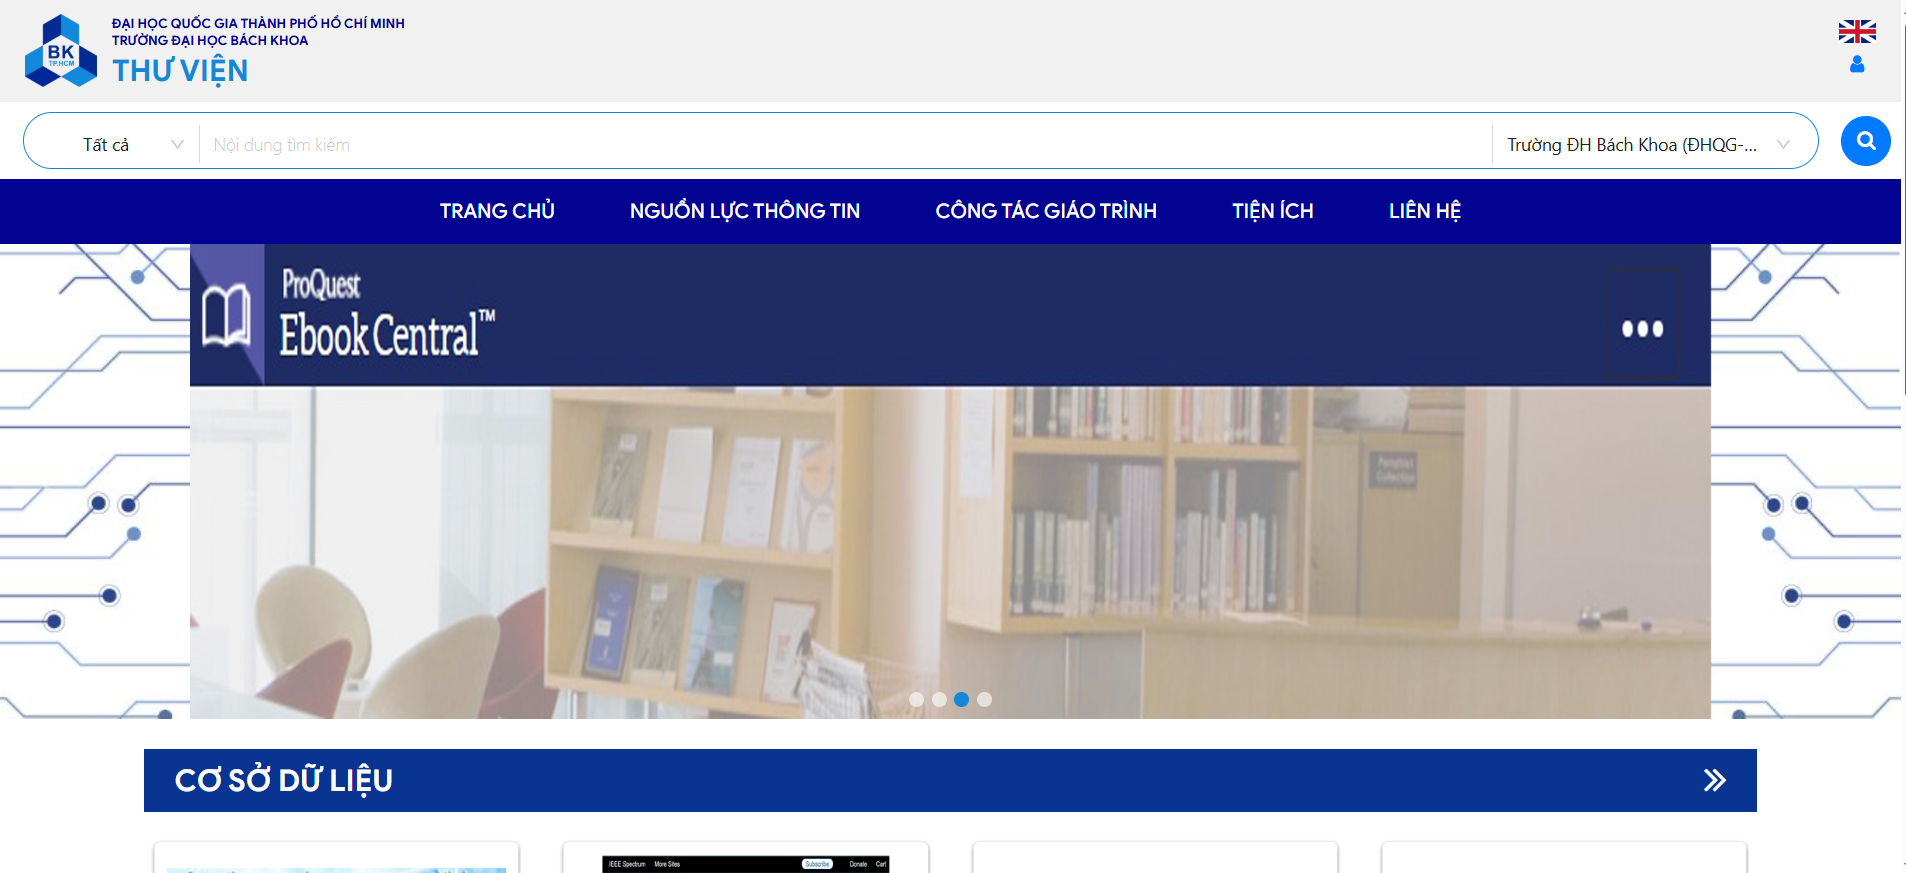
\includegraphics[width=0.8\linewidth]{Images/lib_hcmut_homepage.png} 
     \vspace{10pt}
    \caption{Main interface of the lib.hcmut.edu.vn library portal and print material catalog}
    \label{fig:lib_hcmut_homepage}
\end{figure}

Concurrently, to support in-depth academic research, the university operates the OPAC portal (\url{opac.lib.hcmut.edu.vn}), serving as a specialized search gateway for institutional repository assets. This portal archives and digitizes intellectual assets produced within the university, including student graduation theses, master's theses, doctoral dissertations, and scientific research projects conducted by faculty members. The OPAC interface offers advanced metadata filtering by Author, Advisor, Defense Year, or Academic Field.

The OPAC system is deeply integrated with the university's Single Sign-On authentication system (SSO/BKPay). Upon successfully logging into the "Personal Account" module, readers can manage loan activities such as viewing borrowed items, checking loan histories, tracking overdue fines, requesting loan renewals, or placing holds on items currently checked out.

\begin{figure}[H]
    \centering
    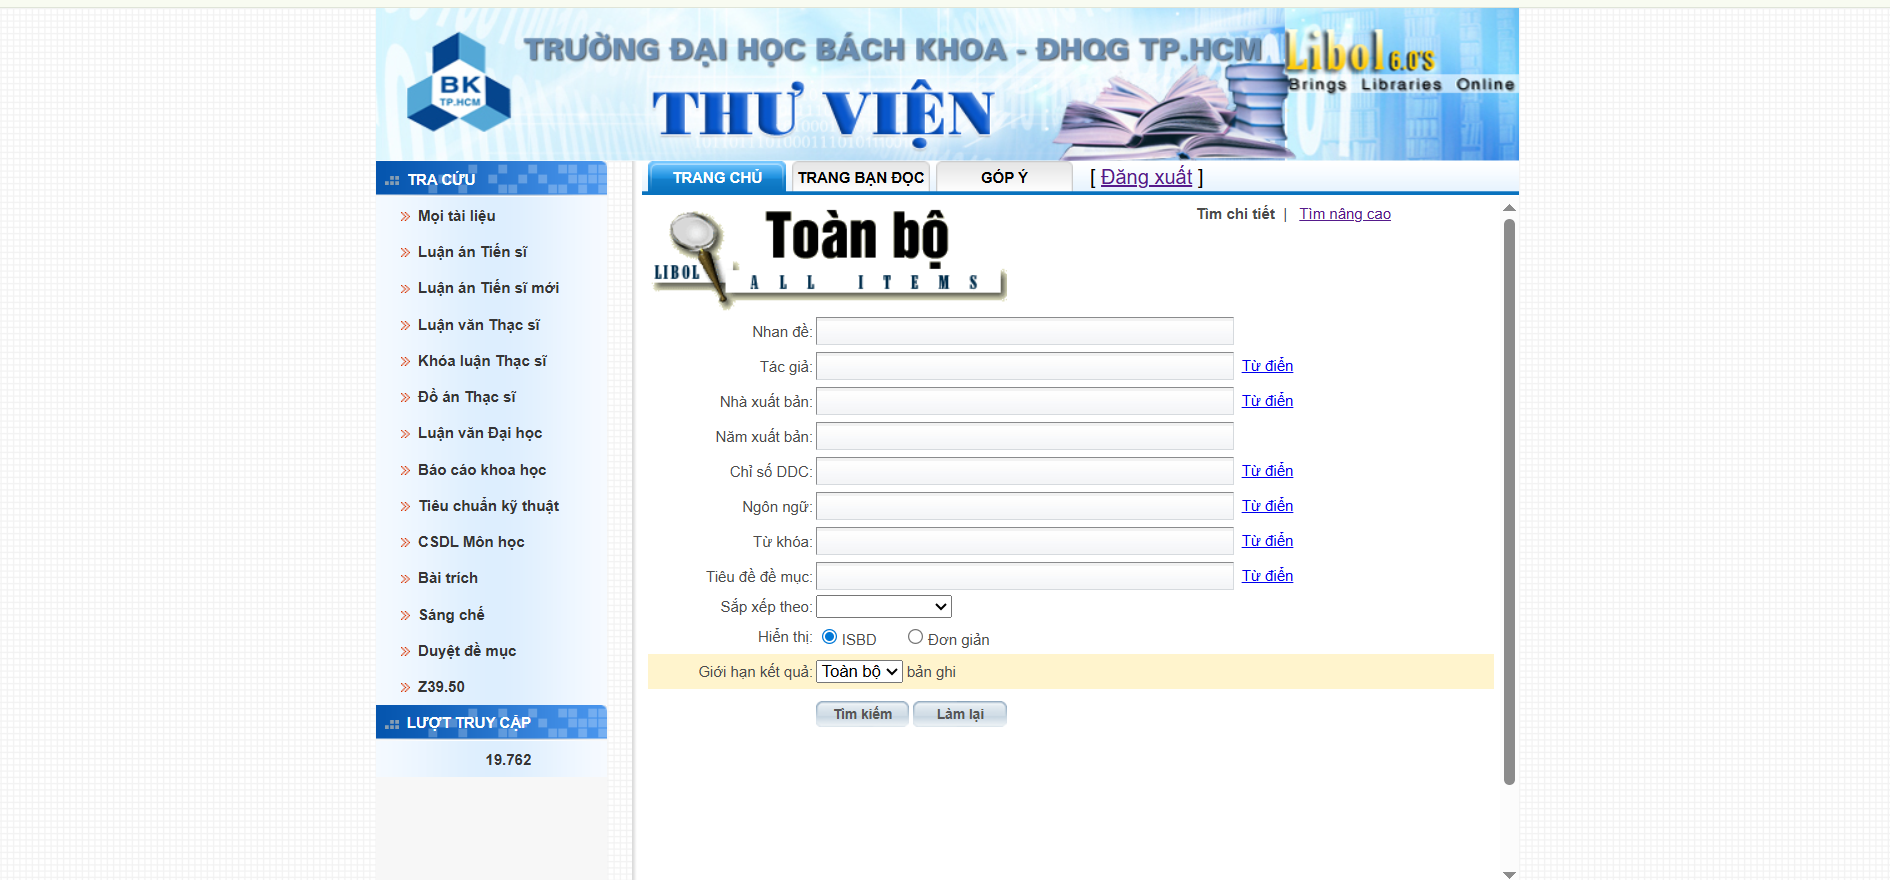
\includegraphics[width=0.8\linewidth]{Images/opac.lib.hcmut.edu.vn.png} 
     \vspace{10pt}
    \caption{Institutional Repository Search Interface and Account Login Module on the OPAC portal}
    \label{fig:opac_hcmut_search}
\end{figure}

Although both portals satisfy core operational needs, data fragmentation between print materials and digital/institutional repositories creates friction in student user experiences. This limitation motivates our team to construct a modern library management system that unifies resource data and optimizes operational workflows through modern software solutions.

\subsubsection{Strengths}
\begin{itemize}
    \item Specialized interface for institutional repositories optimized for querying academic metadata fields.
    \item Online loan-return and hold placement workflows fully compatible with practical library policies.
    \item Single Sign-On (SSO) authentication mechanism synchronizing reader accounts while securing digital resources.
\end{itemize}

\subsubsection{Weaknesses}
\begin{itemize}
    \item Maintaining two independent portals obligates readers to execute repetitive searches across separate domain names.
    \item Search mechanisms rely strictly on exact keyword matching, showing limited natural language understanding.
    \item Static platform architecture lacking automated recommendation features and 24/7 AI virtual assistant tools.
    \item Advanced search interfaces are poorly optimized for mobile devices, exhibiting procedural interaction flows.
\end{itemize}

\subsection{Online Library System -- University of London (The Online Library -- UoL)}

The University of London (UoL) Online Library system at \url{https://onlinelibrary.london.ac.uk/} represents a flagship digital library (E-library) model designed specifically to support global distance-learning students. Unlike traditional physical collection management models, this system operates almost entirely digitally, focusing on managing, storing, and distributing access rights to academic databases, electronic journals (E-journals), and electronic books (E-books).

A key technical highlight of the system is the deployment of a centralized Discovery Service. Rather than requiring users to log into publisher platforms individually, a single unified search bar (One-stop search) retrieves full-text items across hundreds of database sources. Furthermore, to compensate for the absence of in-person assistance, the system features a live support tool ("Chat with us") functioning as a 24/7 help desk to resolve technical inquiries and guide student literature searches.

\begin{figure}[H]
    \centering
     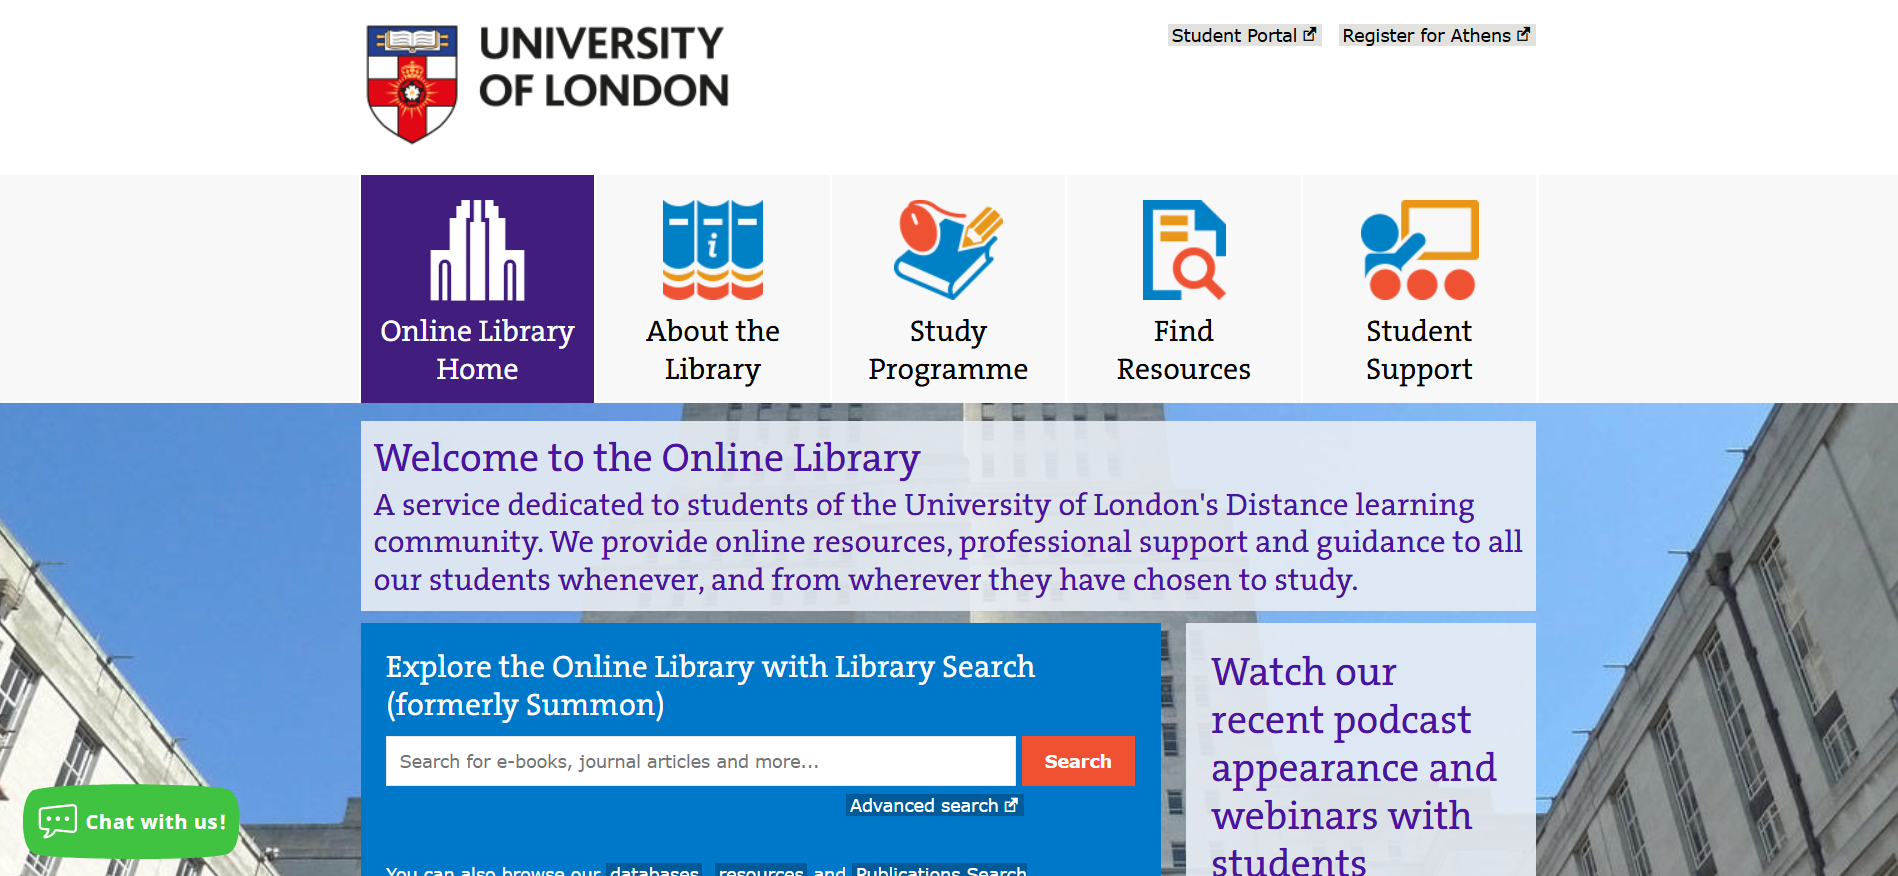
\includegraphics[width=0.8\linewidth]{Images/london_online_library_homepage.png} 
    \vspace{10pt}
    \caption{Unified discovery search interface and live support tool at The Online Library - UoL}
    \label{fig:london_lib_homepage}
\end{figure}

Analyzing the UoL system provides critical insights into optimizing digital user experience while highlighting technological gaps in intelligent algorithmic user interaction.

\subsubsection{Strengths}
\begin{itemize}
    \item Provides a single access gateway for all digital resources, reducing search latency for users.
    \item Employs modern authentication protocols (OpenAthens), enabling seamless remote off-campus access without requiring a VPN.
    \item Categorizes digital materials by specific academic disciplines to guide student literature exploration efficiently.
\end{itemize}

\subsubsection{Weaknesses}
\begin{itemize}
    \item Model is restricted strictly to digital assets, entirely omitting physical book circulation and stack management workflows.
    \item Centralized discovery searching can induce information overload and lacks behavioral analytics for personalized recommendation.
    \item Chatbot support operates on static pre-scripted rules, failing to interpret complex queries and relying heavily on human librarian intervention.
\end{itemize}

\subsection{University of Delaware Library System (UD Library)}

The University of Delaware Library (UD Library) system at \url{https://library.udel.edu/} exemplifies a highly digitized multi-branch university library governance model. Unlike UoL's pure digital focus, UD Library tackles a more complex challenge: managing and distributing data across central and departmental libraries, while pioneering AI virtual assistant integration in student support workflows.

At the core of this system lies \textbf{DELCAT} (Unified Discovery Service), serving as a single interface connecting users with millions of records across diverse formats. Notably, UD Library has begun deploying conversational natural language AI solutions alongside traditional search mechanisms.

\begin{figure}[H]
\centering
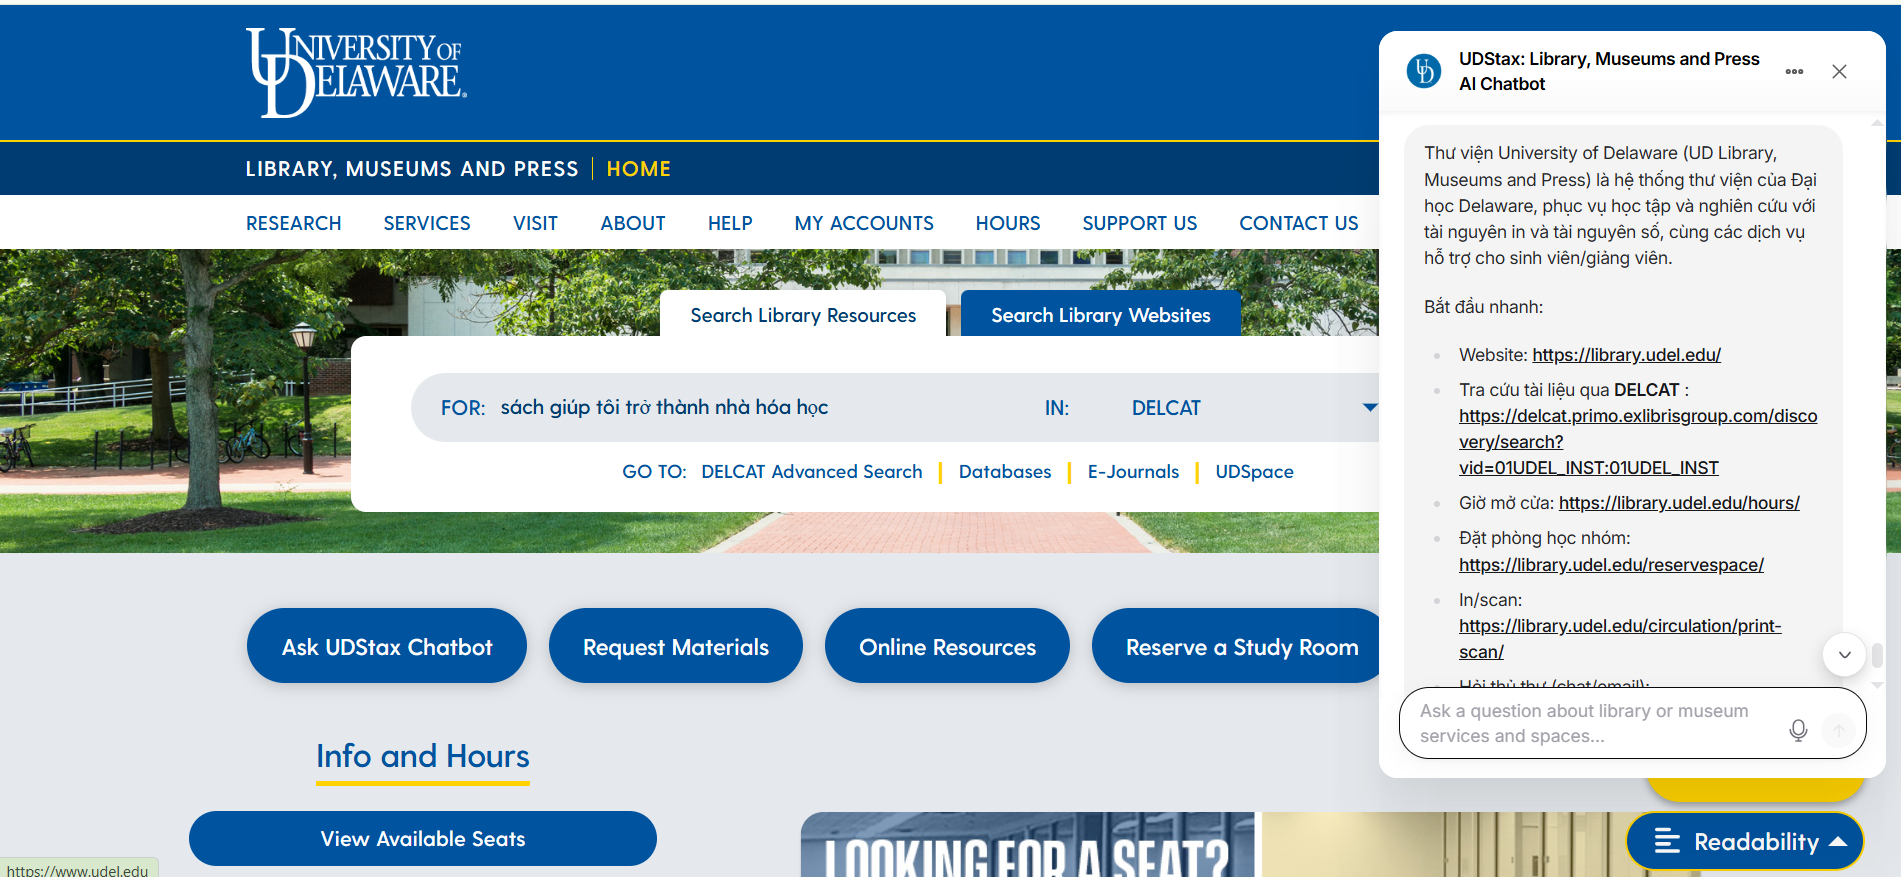
\includegraphics[width=0.8\linewidth]{Images/ud_library_homepage_chatbot.png} 
\vspace{10pt}
\caption{DELCAT unified discovery service interface and supporting AI tool at UD Library}
\label{fig:ud_delcat_search}
\end{figure}

Investigating UD Library offers important architectural perspectives on constructing an "All-in-one" unified discovery platform and operating conversational AI assistants in large academic environments.

\subsubsection{Strengths}
\begin{itemize}
\item Integrates virtual assistants capable of processing natural language to automate routine procedural Q\&A.
\item DELCAT platform unifies print book and electronic resource discovery within a single user interface.
\item Connects non-traditional library services, such as group study room reservations, printing services, and interlibrary loans.
\end{itemize}

\subsubsection{Weaknesses}
\begin{itemize}
\item Chatbot operates independently as a procedural advisory channel without deep integration into search engines for direct book recommendation.
\item Unified discovery architecture frequently causes information overload by returning excessive search result volumes.
\end{itemize}


\subsection{Open Source Library Management System -- Koha ILS}

Koha ILS is the world's most widely adopted open-source Integrated Library System (ILS), utilized by numerous academic institutions and public library networks. Unlike user-facing OPAC portals or Discovery platforms analyzed previously, Koha represents a backend core system focused on digitizing and automating complex administrative workflows for library staff (Librarians).

Through its Staff Client administration portal, Koha offers comprehensive modules for managing physical and digital libraries, including: Circulation, International Cataloging, Patron Management, and Statistical Reporting. Studying Koha provides valuable reference standards for designing database schemas and business rule logic in our project.

\begin{figure}[H]
\centering
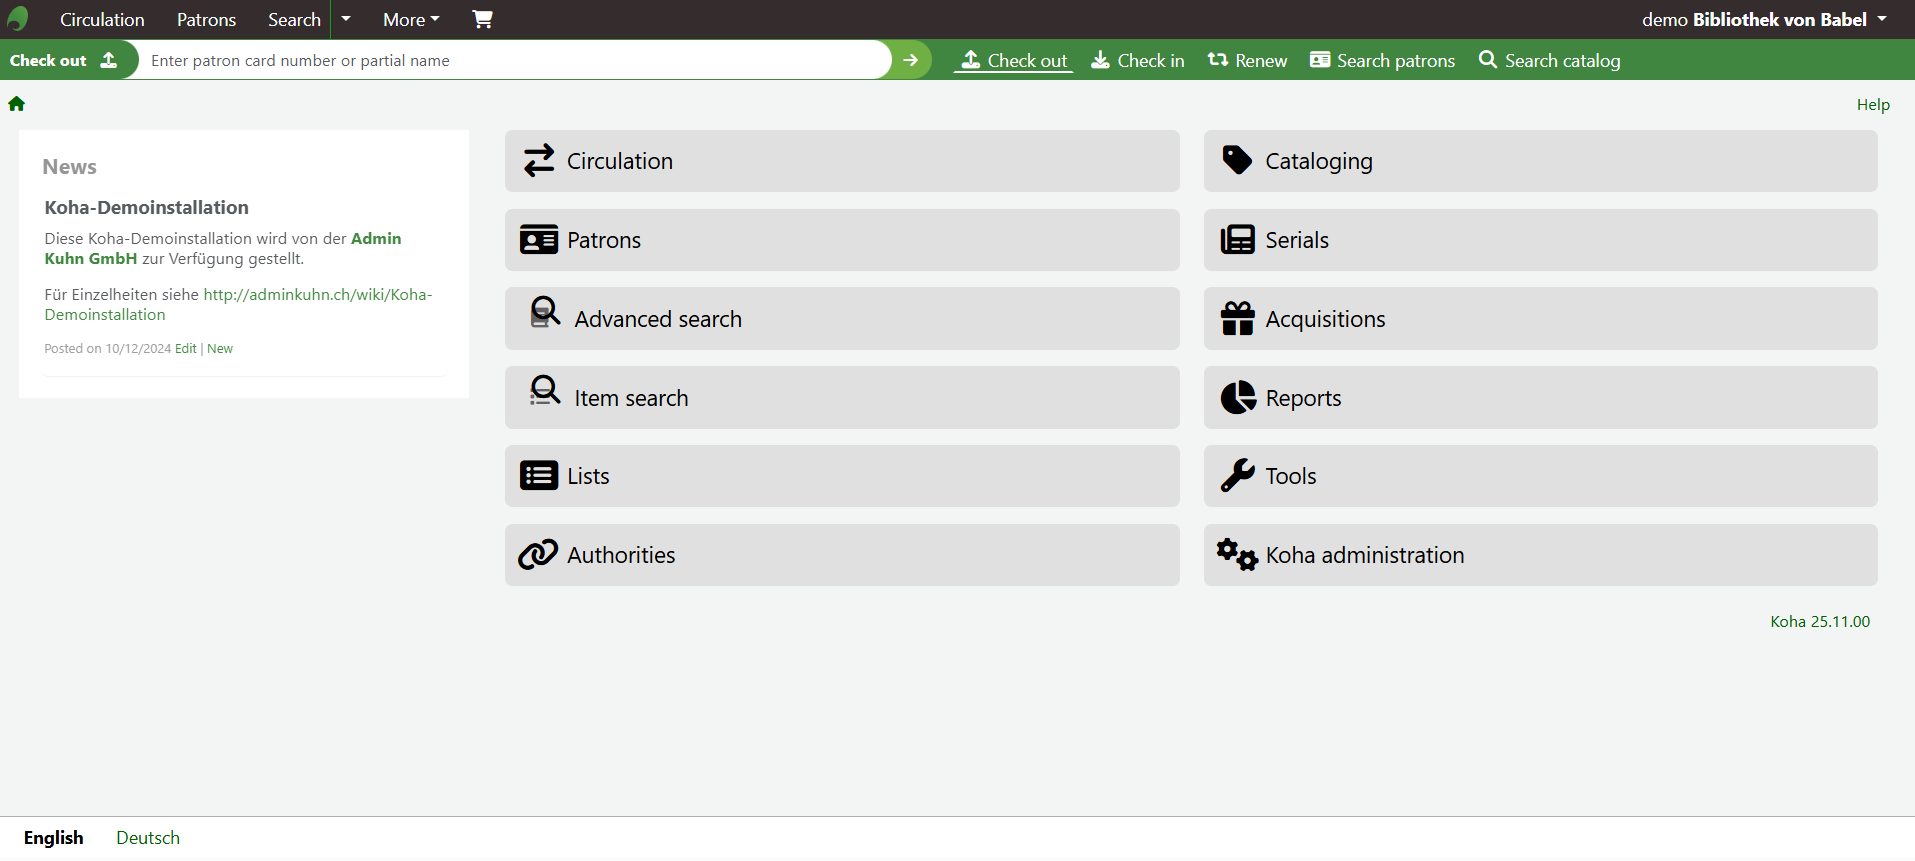
\includegraphics[width=0.8\linewidth]{Images/koha_staff_interface.png} 
\vspace{10pt}
\caption{Koha Staff Client administrative interface module}
\label{fig:koha_admin}
\end{figure}

Analyzing Koha helps clearly delineate essential core features required in library management software while exposing user experience friction present in legacy administrative systems.

\subsubsection{Strengths}
\begin{itemize}
\item Strictly complies with international library metadata standards (MARC21, Z39.50), guaranteeing data consistency and interoperability.
\item Circulation module provides exhaustive rule matrices for configuring borrowing, returning, renewals, and overdue fine logic tailored to user groups.
\item Features built-in REST APIs allowing third-party applications to interact and extract data for platform extension.
\item Reporting system supports direct custom SQL queries, delivering maximum flexibility for administrative reporting.
\end{itemize}

\subsubsection{Weaknesses}
\begin{itemize}
\item Staff Client interface (UI/UX) is verbose, adhering to traditional form-heavy layouts that increase librarian training curves.
\item Data cataloging workflows remain heavily manual, lacking intelligent automated classification or metadata extraction mechanisms.
\item Monolithic system architecture and complex relational database schemas hamper rapid decoupling or custom modular feature additions.
\end{itemize}